\documentclass [12pt,a4paper,twoside]{article}
\usepackage{fullpage}
\usepackage{amssymb,amsmath,amsbsy}
\usepackage[utf8]{inputenc}
\usepackage{fouriernc}
\usepackage[T1]{fontenc}
\usepackage{graphicx}
\usepackage{wrapfig}
\usepackage{subfigure}
\usepackage{setspace}
\usepackage{comment}
\usepackage{float}
%\usepackage{titlesec}
\usepackage[colorlinks]{hyperref}
%\usepackage{bookmark}
\usepackage{indentfirst}
\hypersetup{citecolor=black}
\hypersetup{linkcolor=black}
\usepackage[square,numbers,sort&compress]{natbib}
\hypersetup{pdftitle={An Agent-Based Model of Collective Awareness}}
\hypersetup{pdfauthor={Tamás Kriváchy, Polychronis Patapis}}
\usepackage{fancyhdr}
\usepackage{pdfpages}
\bibliographystyle{ieeetr}

\title{An Agent-Based Model of Collective Awareness}
\author{Tamás Kriváchy, Polychronis Patapis}

\begin{document}


%%%%%%%%%% Begin %%%%%%%%%




\begin{titlepage}
 \begin{center}
   
\includegraphics[width=0.2\textwidth]{report/eth_logo_kurz_pos}\\[1cm]
   {\bf \textsc{\LARGE  An Agent-Based Model of \\[0.1cm] Collective Awareness}}\\[1cm]
   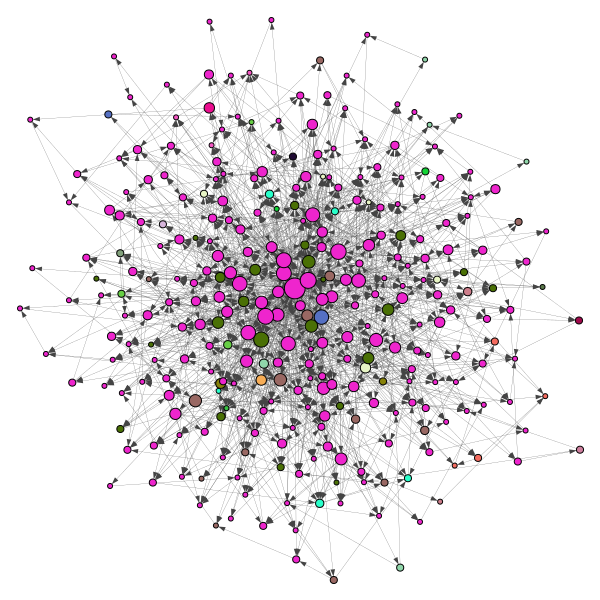
\includegraphics[width=0.8\textwidth]{report/graph}\\[0.1cm]
   {\huge Agent-Based Modelling \\ of Social Systems}\\[1.5cm]
   {\LARGE Tamás Kriváchy}\\
   \LARGE Polychronis Patapis
   %\\[2cm]
 \vfill 
 {\large 06.06.2016} \\
 
 \end{center}
\end{titlepage}

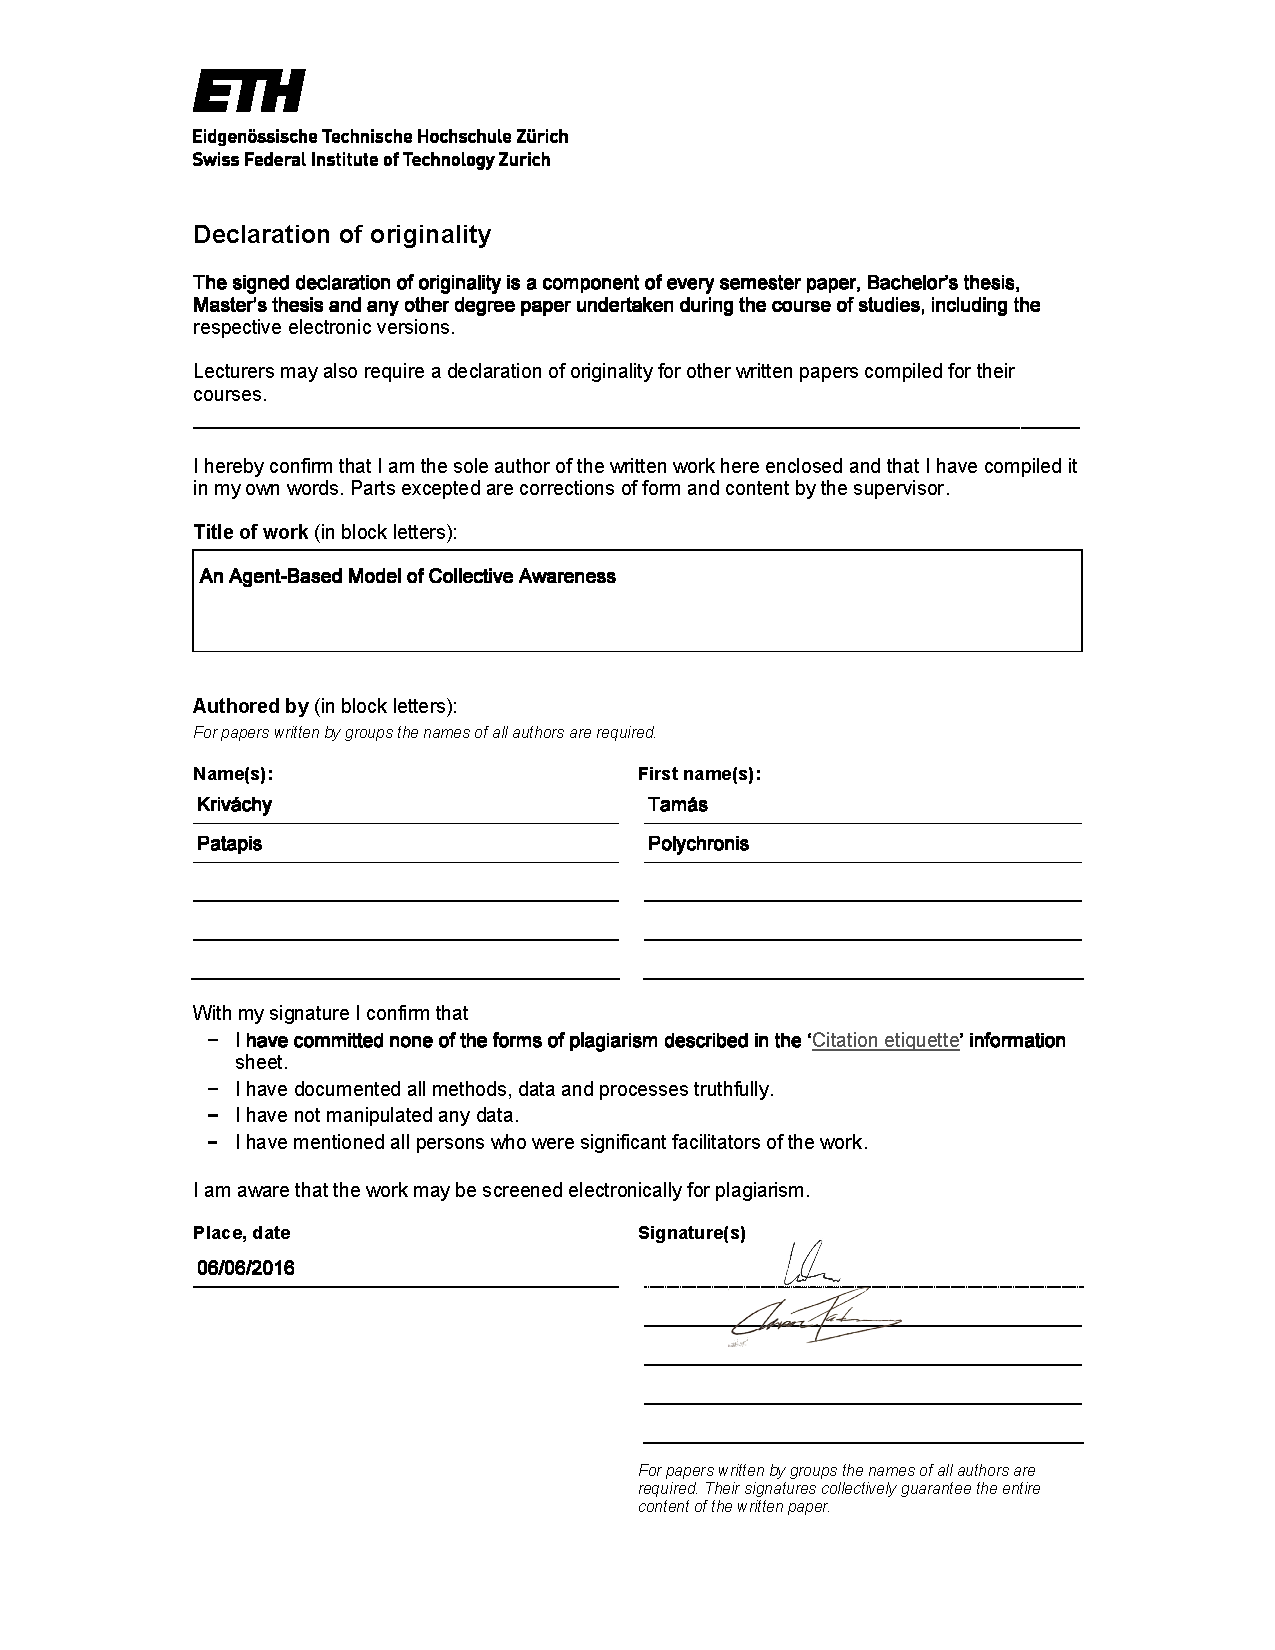
\includepdf{report/Declaration-originality_signed.pdf}

\newpage
\pagestyle{fancy}
  \fancyhead{}
  \headsep = 25pt
  \fancyhead[LE,RO]{\rightmark}
  \fancyhead[LO,RE]{\leftmark}
%  \fancyfoot[C]{\thepage}
\pagenumbering{arabic}
\numberwithin{figure}{section}
\numberwithin{equation}{section}

\section{Motivation}
\subsection{Introduction}
In agent-based modelling, it is often the goal to show that an emergent phenomena arises from simple interactions between agents in a given population. In our project for the 2016 spring semester course "Agent-Based Modelling in Social Systems" at ETH Zürich we decided to try to recreate the phenomena of the collective awareness of a society.

In the scientific community there has been much work on identifying the cause of virality in social networks, as well as on the optimization of marketing strategies to reach virality with a product. Among these, a few are agent-based models, which often analyze the Twitter network and the spreading of information on it \cite{ABM_viral_twitter,ABM_viral_twitter_2,ABM_viral_twitter_3,ABM_viral_twitter_4,ABM_viral_twitter_5,ABM_viral_twitter_6}. These models are usually driven by observations on the network. Contrary to those, our model will build on theoretical assumptions and verify hypotheses.


\subsection{Collective Awareness}

In a state of collective awareness, the majority of a group of people are thinking of the same thing (further referred to as the "event"), and all find it similarly important. In a sense the community as a whole is "aware" of the event at hand.

It is crucial to realize that in the real world events happen at given places and times, and only few people experience the event. Regardless of this, if the event is important, the whole of society will be talking about it, thinking about it and acting on it. An example could be that illegal immigrants enter a country's border and only the communities near the border experience this first-hand, yet the whole country/society talks about the issue.

We can also observe that at some times the awareness of society is directed at an important event, say something to do with national security or central questions in politics, of great relevance to everyone. However, at other times, when nothing "as important" is happening, society becomes aware of much smaller things, e.g. small scandals in politics or the current actions of one celebrity or another. Even though these events are much less important than the events of importance to everyone, they get a similar proportion of attention from the community. In the real world we see an interplay between these more important and less important events - at a given time everyone could be talking and worrying about something, but the next a much more crucial and important event will dominate everyone's discussions. However, when this large event wears off, the masses of people will focus on less important events again.

In real-world societies we consider media to be a broadcaster of information to many people. People working in the media can, on average, reach much more people, than others. What we know as "media", however, is also made up of people, and thus we will consider it as an intrinsic element in our model. Similarly, we all know people who are very popular, and we imagine them to be able to reach much more people than us. In this sense we would expect events that happen to these agents to become globally discussed more easily.

A summary of phenomena related to collective awareness in societies that we want to observe follows.
\begin{itemize}
\item Events happening locally at an individual, but being discussed globally by the majority of the society.
\item The eventual loss of interest, and forgetting of events that happened at earlier times.
\item The interplay between discussion very important events and of less significant events in times when there are no important events to discuss.
\item The importance of people who can broadcast information to many people ("the media").
\item Observation of how important the location of an agent is in the network.
\end{itemize}

\subsection{The Global Workspace Model}

The main motivation for making our model is the observation of collective awareness, a phenomena that is not just present in societies, but also in human beings. Our brains are composed of countless neurons that process electrical signal individually, yet in the end the result is a conscious mind. Since the phenomena of consciousness is so similar to that of social collective awareness, we decided to take intuition from the field of psychology and neuroscience, whose subfields study these questions. In particular we will be focusing on a particular model, the global workspace model (GW), and its neuroscience counterpart, the neural global workspace model (NGW). At this point we would like to point out that in the scientific community the awareness of the brain is usually taken to be as a subphenomena of consciousness. In particular awareness can arise without consciousness arising. When examining social systems we are also not trying to find consciousness, just collective awareness.

The GW model was originally a psychological model of the functioning of the brain. The model states that there is a global workspace of the mind, where some content is worked on. Whatever is currently in the global workspace is broadcasted to the rest of the mind. In this sense the global workspace is the conscious part of our thinking, and the rest is the unconscious. The simplest way to visualize the GW model is to imagine a theater play. The stage is the global workspace, the actors on the stage are the few things that the an individual is "keeping in mind" at the moment. The spotlight shines on one of these actors, and the whole audience receives information from that actor. Actors compete to get on the stage and to get into the spotlight. The audience just receives information and processes it. A schematic representation of the GW model can be seen on fig. \ref{global_workspace}.

\begin{figure}[h!]
  \centering
  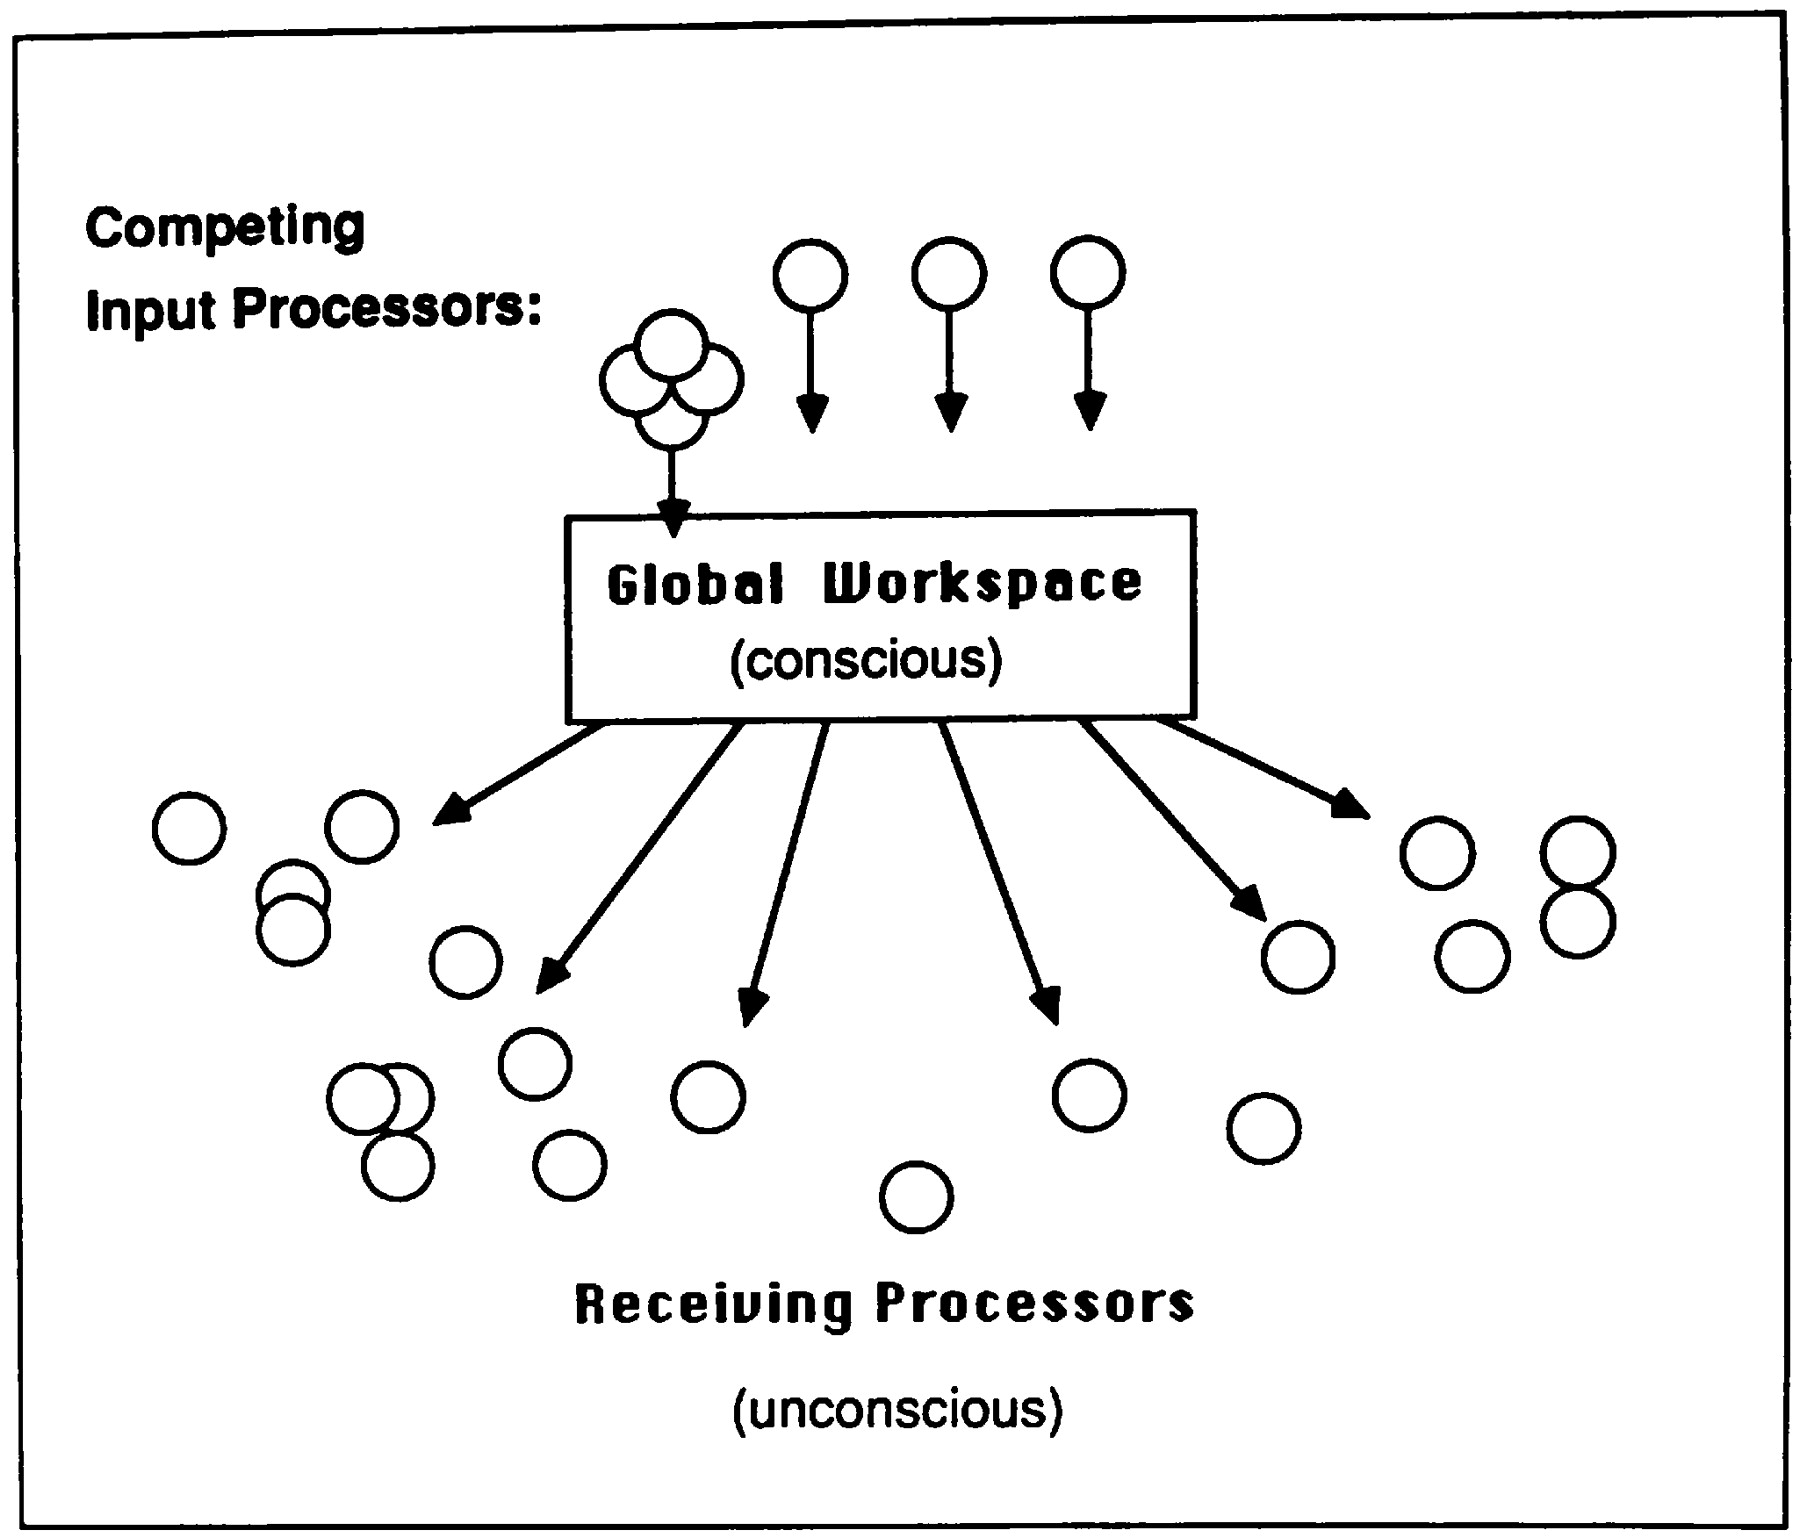
\includegraphics[width=0.45\linewidth]{report/GW_schematic.jpg}
  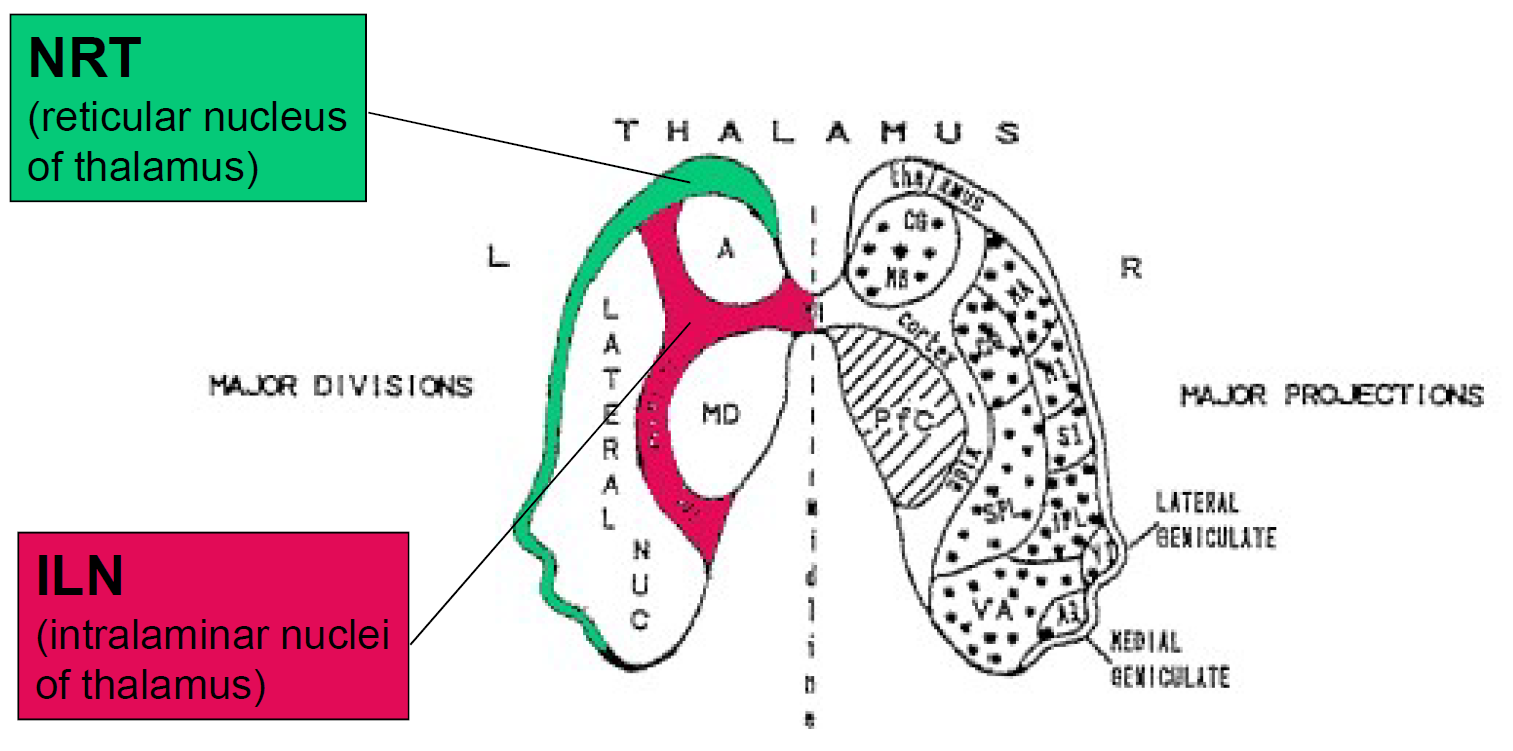
\includegraphics[width=0.54\linewidth]{report/thalamus.png}
  \caption{Left: Schematic interpretation of the global workspace model. Right: cross-section of the thalamus.}
  \label{global_workspace}
\end{figure}

The intriguing thing about the GW model is that years after its conception, findings in neuroscience showed that the neural connections in the brains naturally display a similar structure as what the GW model suggests. The GW model based on neural connections is often referred to as the neural global workspace model (NGW model). In the NGW, the corresponding parts of the brain for the GW model have to be found. The functions of competition for access to consciousness, selection of content for consciousness and global broadcasting of this content is fulfilled in the brain by the brainstem reticular formation (RF) and two parts of the thalamus: the reticular nucleus (NRT) and intralaminar nuclei (ILN). A cross section of the thalamus can be seen in fig. \ref{global_workspace}. The RF receives all major sensory and motor input from the brain, and conveys much of it to the thalamus. The thalamus has parts which project to specific areas of the cortex, but also a part, the ILN, which project diffusely to the rest of the brain. The NRT surrounds the thalamus, and much of the information passes through it. It can and must "gate" the outgoing information, since there is large competition in all different kinds of stimuli. In some way this function corresponds to the spotlight in the GW. \cite{lecture-notes}

What part of the GW and NGW model do we want to use in our model of social collective awareness? Both models describe consciousness by having a central core (the global workspace) which is able to broadcast to the rest of the brain/mind. The content of the broadcasting, however, is determined by a competition between content coming from the whole of the brain/mind. This has a natural implementation in social networks, where we expect a small core of people to be able to broadcast to the large masses, which the content they broadcast is, in general, generated by the peripheral agents.


\section{The Model}


\section{Results, Discussion}

\section{Conclusion}
In the paper \cite{Similar-results}, the analyzed real data with machine learning algorithms, and came to the conclusion that for content to become viral through Twitter, the content itself has to be good, and the location of initializing agents on the network are much less important. This is in accordance to our findings, that in societies with a high tech-parameter (such as the society of people using Twitter), the quality of the content is important for it to get into the collective awareness.

\section{Outlook}
It would be important to include community structure. According to \cite{Virality-community-important}, virality of a meme on the internet can be much better predicted if one takes into account whether content spreads easily from cluster to cluster or not.

%%% PUT \small \setlength{\bibsep}{0pt} IN BBL FILE
\small \setlength{\bibsep}{1pt}
\bibliographystyle{Collective_Awareness_2016-style}
%\bibliographystyle{apa}
\bibliography{Collective_Awareness_2016}

\end{document}